\chapter{Scaling FDTD Simulations to Any Frequency
 \label{chap:dimensionless}}

%\setcounter{page}{1}

\renewcommand{\thefootnote}{\fnsymbol{footnote}}
\footnotetext{Lecture notes by John Schneider.  {\tt
fdtd-dimensionless.tex}}

\section{Introduction}

The FDTD method requires the discretization of time and space.
Samples in time are $\Delt$ apart whereas, in simulations with one
spatial dimension, samples in space are $\Delx$ apart.  It thus
appears that one must specify $\Delt$ and $\Delx$ in order to perform
a simulation.  However, as shown in Sec.\ \ref{sec:update}, it is
possible to write the coefficients $\Delt/\epsilon\Delx$ and
$\Delt/\mu\Delx$ in terms of the material parameters and the Courant
number (ref.\ \refeq{eq:coefEz} and \refeq{eq:coefHy}).  Since the
Courant number contains the ratio of the temporal step to the spatial
step, it allows one to avoid explicitly stating a definite temporal or
spatial step---all that matters is their ratio.  This chapter
continues to examine ways in which FDTD simulations can be treated as
generic simulations that can be scaled to any size/frequency.  As will
be shown, the important factors which dictate the behavior of the
fields in a simulation are the Courant number and the points per
wavelength for any given frequency.  We conclude the chapter by
considering how one can obtain the transmission coefficient for a
planar interface from a FDTD simulation.

\section{Sources}

\subsection{Gaussian Pulse}

In the previous chapter the source function, whether hardwired,
additive, or incorporated in a TFSF formulation, was always a
Gaussian.  In the continuous world this function can be expressed as
\begin{equation}
  f_g(t) = e^{-\left(\frac{t - d_g}{w_g}\right)^2}
  \label{eq:gaussianGeneric}
\end{equation}
where $d_g$ is the temporal delay and $w_g$ is a pulse-width
parameter.  The Gaussian has its peak value at $t=d_g$ (when the
exponent is zero) and has a value of $e^{-1}$ when $t=d_g\pm w_g$.
Since \refeq{eq:gaussianGeneric} is only a function of time, i.e., a
function of $q\Delt$ in the discretized world, it again appears as if
the temporal step $\Delt$ must be given explicitly.  However, if one
specifies the delay and pulse width in terms of temporal steps, the
term $\Delt$ appears in both the numerator and the denominator of the
exponent.  For example, in the last chapter $d_g$ was $30\Delt$ and
$w_g$ was $10\Delt$ so the source function could be written
\begin{equation}
   f_g(q\Delt) = f_g[q] = e^{-\left(\frac{q - 30}{10}\right)^2}.
\end{equation}
Note that $\Delt$ does not appear on the right-hand side.  

The discretized version of a function $f(q\Delt)$ will be written
$f[q]$, i.e., the temporal step will be dropped from the argument
since it does not appear explicitly in the expression for the function
itself.  The key to being able to discard $\Delt$ from the source
function was the fact that the source parameters were expressed in
terms of the number of temporal steps.

\subsection{Harmonic Sources \label{sec:harmonicSources}}

For a harmonic source, such as
\begin{equation}
  f_h(t)=\cos(\omega t),
\end{equation}
there is no explicit numerator and denominator in the argument.
Replacing $t$ with $q\Delt$ it again appears as if the temporal step
must be given explicitly.  However, keep in mind that with
electromagnetic fields there is an explicit relationship between
frequency and wavelength.  For a plane wave propagating in free space,
the wavelength $\lambda$ and frequency $f$ are related by
\begin{equation}
  f \lambda=c \qquad\Rightarrow \qquad f=\frac{c}{\lambda}.
\end{equation}
Thus the argument $\omega t$ (i.e., $2 \pi f t$) can also be written
as
\begin{equation}
  \omega t = \frac{2\pi c}{\lambda}t.
\end{equation}
For a given frequency, the wavelength is a fixed length.  Being a
length, it can be expressed in terms of the spatial step, i.e.,
\begin{equation}
  \lambda = \ppw \Delx
\end{equation}
where $\ppw$ is the number of points per wavelength.  This does not
need to be an integer.

By relating frequency to wavelength and the wavelength to $\ppw$, the
discretized version of the harmonic function can be written
\begin{equation}
 f_h(q\Delt) = \cos\!\left(\frac{2 \pi c}{\ppw\Delx} q \Delt\right)
           = \cos\!\left(\frac{2 \pi}{\ppw}\frac{c\Delt}{\Delx} q\right),
 \label{eq:fHarmonic}
\end{equation}
or, simply,
\begin{equation}
   f_h[q] = \cos\!\left(\frac{2 \pi S_c}{\ppw} q\right).
 \label{eq:fHarmonicI}
\end{equation}
The expression on the right now contains the Courant number and the
parameter $\ppw$.  In this form one does not need to state an explicit
value for the temporal step.  Rather, one specifies the Courant
number $S_c$ and the number of spatial steps per wavelength $\ppw$.
Note that $\ppw$ we will always be defined in terms of the number of
spatial steps per the wavelength in free space.  Furthermore, the
wavelength is the one in the continuous world---we will see later that
the wavelength in the FDTD grid is not always the same.

The period for a harmonic function is the inverse of the frequency
\begin{equation}
  T = \frac{1}{f} = \frac{\lambda}{c} = \frac{\ppw\Delx}{c}.
\end{equation}
The number of time steps in a period is thus given by
\begin{equation}
  \frac{T}{\Delt} = \frac{\ppw\Delx}{c\Delt} = \frac{N_\lambda}{S_c}.
\end{equation}

A harmonic wave traveling in the positive $x$ direction is given by
\begin{equation}
  f_h(x,t) = \cos(\omega t - k x) = 
  \cos\!\left(\omega\left(t - \frac{k}{\omega} x\right)\right).
  \label{eq:harmonicTravel}
\end{equation}
Since $k=\omega\sqrt{\mu_0\mu_r\epsilon_0\epsilon_r}=
\omega\sqrt{\mu_r\epsilon_r}/c$, the argument can be written
\begin{equation}
  \omega\left(t - \frac{k}{\omega} x\right) =
  \omega\left(t - \frac{\sqrt{\mu_r\epsilon_r}}{c} x\right).
\end{equation}
Expressing all quantities in terms of the discrete values which
pertain in the FDTD grid yields
\begin{equation}
  \omega\left(t - \frac{\sqrt{\mu_r\epsilon_r}}{c} x\right) =
    \frac{2\pi c}{\ppw\Delx}
    \left(q\Delt - \frac{\sqrt{\mu_r\epsilon_r}}{c} m\Delx\right) =
        \frac{2\pi}{\ppw}(S_c q - \sqrt{\mu_r\epsilon_r}m).
\end{equation}
Therefore the discretized form of \refeq{eq:harmonicTravel} is given
by
\begin{equation}
  f_h[m,q] =
    \cos\!\left(\frac{2\pi}{\ppw}
                \left(S_c q-\sqrt{\mu_r\epsilon_r}m\right)\right).
\end{equation}
This equation could now be used as the source in a
total-field/scattered-field implementation.  (However, note that when
the temporal and spatial indices are zero this source has a value of
unity.  If that is the initial ``turn-on'' value of the source, that
may cause artifacts which are undesirable.  This will be considered
further when dispersion is discussed.  It is generally better to ramp
the source up gradually.  A simple improvement is offered by using a
sine function instead of a cosine since sine is initially zero.)

\subsection{The Ricker Wavelet \label{sec:ricker}}

One of the features of the FDTD technique is that it allows the
modeling of a broad range of frequencies using a single simulation.
Therefore it is generally advantageous to use pulsed sources---which
can introduce a wide spectrum of frequencies---rather than a harmonic
source.  The Gaussian pulse is potentially an acceptable source except
that it contains a dc component.  In fact, for a Gaussian pulse dc is
the frequency with the greatest energy.  Generally one would not use
the FDTD technique to model dc fields.  Sources with dc components
also have the possibility of introducing artifacts which are not
physical (e.g., charges which sit in the grid).  Therefore we consider
a different pulsed source which has no dc component and which can have
its most energetic frequency set to whatever frequency (or
discretization) is desired.

The Ricker wavelet is equivalent to the second derivative of a
Gaussian; it is simple to implement; it has no dc component; and, its
spectral content is fixed by a single parameter.  The Ricker wavelet
is often written
\begin{equation}
f_r(t) = \left(1-2 \bigl\{\pi f_P \left[t-d_r\right]\bigr\}^2\right)
         \exp\!\left(-\bigl\{\pi f_P \left[t-d_r\right]\bigr\}^2\right)
\label{eq:rickerTime}
\end{equation}
where $f_P$ is the ``peak frequency'' and $d_r$ is the temporal delay.
As will be more clear when the spectral representation of the function
is shown below, the peak frequency is the frequency with the greatest
spectral content.

The delay $d_r$ can be set to any desired amount, but it is convenient
to express it as a multiple of $1/f_P$, i.e.,
\begin{equation}
  d_r = M_d \frac{1}{f_P}
\end{equation}
where $M_d$ is the delay multiple (which need not be an integer).  An
FDTD simulation is typically assumed to start at $t=0$, but $f_r(t)$
is not zero for $t<0$---rather $f_r(t)$ asymptotically approaches zero
for large and small values of the argument, but never actually reaches
zero (other than at two discrete zero-crossings).  However, with a
delay of $d_r=1/f_P$ (i.e., $M_d=1$), $|f_r(t<0)|$ is bound by
$0.001$, which is small compared to the peak value of unity.  Thus,
the transient caused by ``switching on'' $f_r(t)$ at $t=0$ is
relatively small with this amount of delay.  Said another way, since
the magnitude of $f_r(t)$ is small for $t<0$, these values can be
approximated by assuming they are zero.  For situations that may
demand a smoother transition (i.e., a smaller initial turn-on value),
the bound on $|f_r(t<0)|$ can be made arbitrarily small by increasing
$d_r$.  For example, with a delay multiple $M_d$ of $2$, $|f_r(t<0)|$
is bound by $10^{-15}$.

The Fourier transform of \refeq{eq:rickerTime} is
\begin{equation}
  F_r(\omega) = -\frac{2}{f_P\sqrt{\pi}}
           \left(\frac{\omega}{2\pi f_P}\right)^2
           \exp\!\left(-jd_r\omega
	             -\left[\frac{\omega}{2\pi f_P}\right]^2\right).
  \label{eq:rickerOmega}
\end{equation}
Note that the delay $d_r$ only appears as the imaginary part of the
exponent.  Thus it affects only the phase of $F_r(\omega)$, not the
magnitude.

The functions $f_r(t)$ and $|F_r(\omega)|$ are shown in Fig.\
\ref{fig:p-of-t-and-omega}.  For the sake of illustration, $f_P$ is
arbitrarily chosen to be $1$ Hz and the delay is $1$ s.  Different
values of $f_P$ change the horizontal scale but they do not change the
general shape of the curve.  To obtain unit amplitude at the peak
frequency, $F_r(\omega)$ has been scaled by $f_P e\sqrt{\pi}/2$.
\begin{figure}
  \begin{center}
    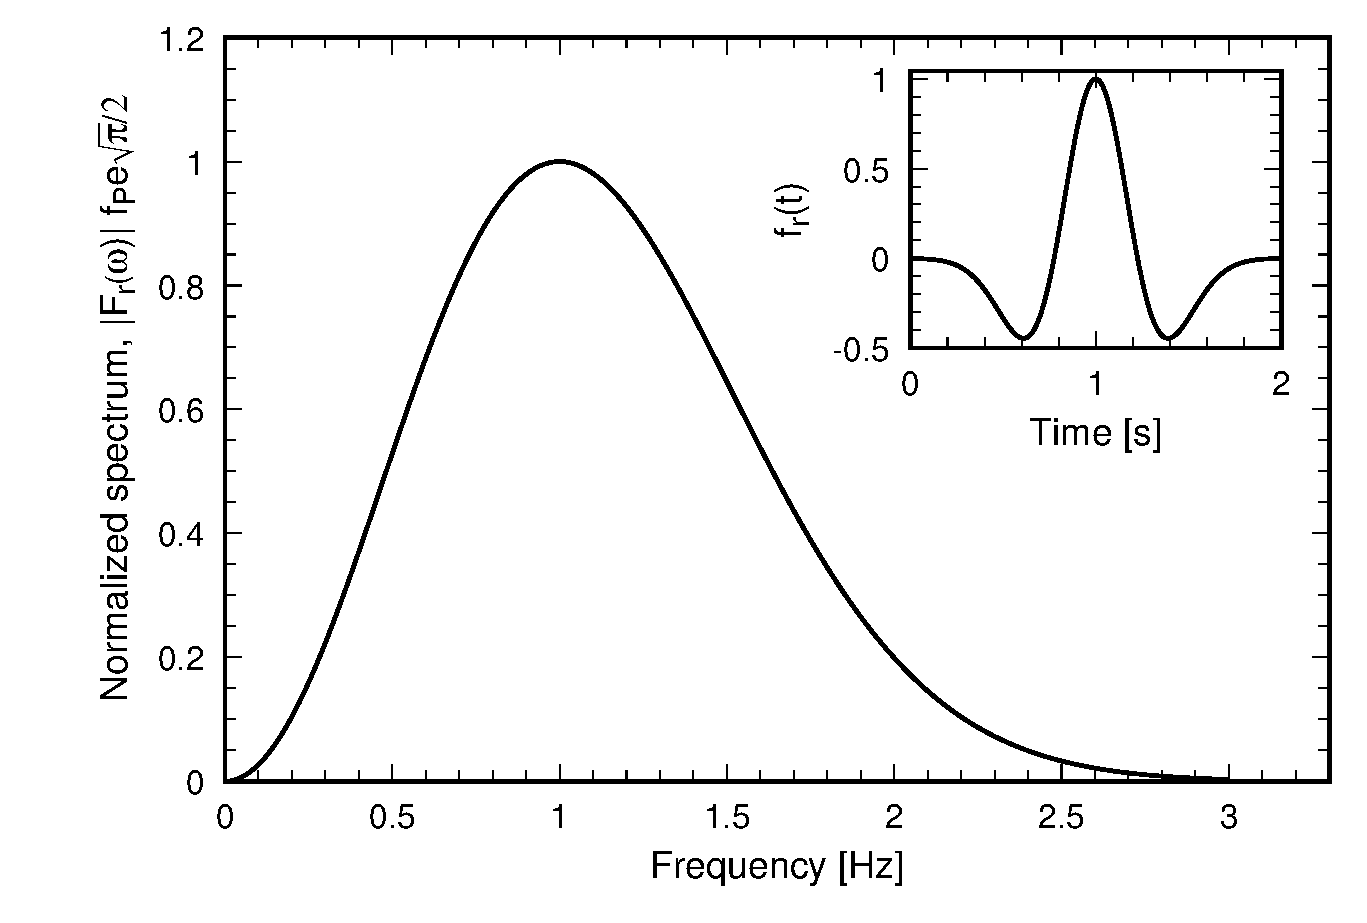
\epsfig{width=4.75in,%
            file=Figures/Fdtd-dimensionless/ricker-freq-time-print.eps}
  \end{center}
  \vspace{-.25in}
  \caption{Normalized spectrum of the Ricker wavelet with $f_P = 1$
  Hz.  The corresponding temporal form $f_r(t)$ is shown in the inset
  box where a delay of $1$ s has been assumed.  For other values of
  $f_P$, the horizontal axis in the time 
  domain is scaled by $1/f_P$.  For example, if $f_P$ were $1$ MHz,
  the peak would occur at $1$ $\mu$s rather than at $1$ s.  In the
  spectral domain, the horizontal axis is directly scaled by $f_P$ so
  that if $f_P$ were $1$ MHz, the peak would occur at $1$ MHz.}
  \label{fig:p-of-t-and-omega}
\end{figure}

The peak frequency $f_P$ has a corresponding wavelength $\lambda_P$.
This wavelength can be expressed in terms of the spatial step such
that $\lambda_P = N_P\Delx$, where $N_P$ does not need to be an
integer.  Thus
\begin{equation}
  f_P = \frac{c}{\lambda_P} = \frac{c}{N_P \Delx}
  \label{eq:peakExpression}
\end{equation}
The Courant number $S_c$ is $c\Delt/\Delx$ so the spatial step can be
expressed as $\Delx = c \Delt/S_c$.  Using this in
\refeq{eq:peakExpression} yields
\begin{equation}
  f_P = \frac{S_c}{N_P \Delt}.
  \label{eq:fp-equiv}
\end{equation}
The delay can thus be expressed as
\begin{equation}
  d_r = M_d\frac{1}{f_P} = M_d \frac{N_P \Delt}{S_c}.
 \label{eq:dr-equiv}
\end{equation}
Letting time $t$ be $q\Delt$ and expressing $f_P$ and $d_r$ as in
\refeq{eq:fp-equiv} and \refeq{eq:dr-equiv}, the discrete form of
\refeq{eq:rickerTime} can be written
as
\begin{equation}
  f_r[q] =
  \left(1-
  2 \pi^2 \left[\frac{S_c q}{N_P} - M_d\right]^2\right)
  \exp\left(-\pi^2 \left[\frac{S_c q}{N_P} - M_d\right]^2\right).
  \label{eq:rickerDiscrete}
\end{equation}
Note that the parameters that specify $f_r[q]$ are the Courant number
$S_c$, the points per wavelength at the peak frequency $N_P$, and the
delay multiple $M_d$---there is no $\Delt$ in
\refeq{eq:rickerDiscrete}.  This function appears to be independent of
the temporal and spatial steps, but it does depend on their ratio via
the Courant number $S_c$.

Equation \refeq{eq:rickerTime} gives the Ricker wavelet as a function
of only time.  However, as was discussed in Sec.\ \ref{sec:tfsf}, when
implementing a total-field/scattered-field boundary, it is necessary
to parameterize an incident field in both time and space.  As shown in
Sec.\ \ref{sec:waveEq}, one can always obtain a traveling plane-wave
solution to the wave equation simply by tweaking the argument of any
function that is twice differentiable.  Given the Ricker wavelet
$f_r(t)$, $f_r(t\pm x/c)$ is a solution to the wave equation where $c$
is the speed of propagation.  The plus sign corresponds to a wave
traveling in the negative $x$ direction and the negative sign
corresponds to a wave traveling in the positive $x$ direction.
(Although only 1D propagation will be considered here, this type
of tweaking can also be done in 2D and 3D.)  Therefore, a traveling
Ricker wavelet can be constructed by replacing the argument $t$ in
\refeq{eq:rickerTime} with $t\pm x/c$.  The value of the function now
depends on both time and location, i.e., it is a function of two
variables:
\begin{eqnarray}
f_r(t\pm x/c) & = & f_r(x,t), \nonumber \\
& = & \left(1-2 \pi^2 f_P^2 \left[t\pm\frac{x}{c}-d_r\right]^2\right)
       \exp\left(-\pi^2 f_P^2 \left[t\pm\frac{x}{c}-d_r\right]^2\right).
\end{eqnarray}
As before, \refeq{eq:dr-equiv} and \refeq{eq:fp-equiv} can be used to
rewrite $d_r$ and $f_P$ in terms of the Courant number, the points per
wavelength at the peak frequency, the temporal step, and the delay
multiple.  Replacing $t$ with $q\Delt$, $x$ with $m\Delx$, and
employing the identity $x/c = m\Delx/c = m\Delt/S_c$, yields
\begin{equation}
  f_r[m,q] =
  \left(1 - 2 \pi^2 \left[\frac{S_c q\pm m}{N_P} - M_d\right]^2\right)
  \exp\left(-\pi^2 \left[\frac{S_c q\pm m}{N_P} - M_d\right]^2\right).
  \label{eq:rickerDiscretex} 
\end{equation}
This gives the value of the Ricker wavelet at temporal index $q$ and
spatial index $m$.  Note that when $m$ is zero \refeq{eq:rickerDiscretex}
reduces to \refeq{eq:rickerDiscrete}.


\section{Mapping Frequencies to Discrete Fourier Transforms
\label{sec:fftMapping}}

Assume the field was recorded during an FDTD simulation and then the
recorded field was transformed to the frequency domain via a discrete
Fourier transform.  The discrete transform will yield a set of complex
numbers that represents the amplitude of discrete spectral components.
The question naturally arises: what is the correspondence between the
indices of the transformed set and the actual frequency?

In any simulation, the highest frequency $f_{\mathrm{max}}$ that can
exist is the inverse of the shortest period that can exist.  In a
discrete simulation one must have at least two samples per period.
Since the time samples are $\Delt$ apart, the shortest possible period
is $2\Delt$.  Therefore
\begin{equation}
  f_{\mathrm{max}} = \frac{1}{2\Delt}.
  \label{eq:fMax}
\end{equation}
The change in frequency from one discrete frequency to the next is the
spectral resolution $\Delf$.  The spectral resolution is dictated
by the total number of samples which we will call $N_T$ (an integer
value).  In general $N_T$ would correspond to the number of time steps
in an FDTD simulation.  The spectral resolution is given by
\begin{equation}
  \Delf = \frac{f_{\mathrm{max}}}{N_T/2}.
  \label{eq:delF}
\end{equation}
The factor of two is a consequence of the fact that there are both
positive and negative frequencies.  Thus one can think of the entire
spectrum as ranging from $-f_{\mathrm{max}}$ to $f_{\mathrm{max}}$,
i.e., an interval of $2f_{\mathrm{max}}$ which is then divided by
$N_T$.  Alternatively, to find $\Delf$ we can divide the maximum
positive frequency by $N_T/2$ as done in $\refeq{eq:delF}$.  Plugging
\refeq{eq:fMax} into \refeq{eq:delF} yields
\begin{equation}
  \Delf = \frac{1}{N_T\Delt}.
\end{equation}

In Sec.\ \ref{sec:harmonicSources} it was shown that a given frequency
$f$ could be written $c/\lambda=c/\ppw\Delx$ where $\ppw$ is the
number of points per wavelength (for the free-space wavelength).
After transforming to the spectral domain, this frequency would have a
corresponding index given by
\begin{equation}
  N_{\mathrm{freq}} = \frac{f}{\Delf} 
  = \frac{N_T c \Delt}{\ppw\Delx} 
  = \frac{N_T}{\ppw} \frac{c \Delt}{\Delx}
  = \frac{N_T}{\ppw} S_c.
  \label{eq:spectralIndex}
\end{equation}
Thus, the spectral index is dictated by the duration of the simulation
$N_T$, the Courant number $S_c$, and the points per wavelength $\ppw$.

Note that in practice different software packages may index things
differently.  The most typical practice is to have the first element
in the spectral array correspond to dc, the next $N_T/2$ elements
correspond to the positive frequencies, and then the next $(N_T/2)-1$
elements correspond to the negative frequencies (which will always be
the complex conjugates of the positive frequencies in any real FDTD
simulation).  The negative frequencies typically are stored from
highest frequency to lowest (i.e., fastest varying to slowest) so that
the last value in the array corresponds to the negative frequency
closest to dc ($-\Delf$).  Additionally, note that in 
\refeq{eq:spectralIndex} dc corresponds to an $N_{\mathrm{freq}}$ of
zero (since $\ppw$ is infinity for dc).  However when using Matlab the
dc term in the array obtained using the {\tt fft()} command has an
index of one.  The first element in the array has an index of
one---there is no ``zero'' element in Matlab arrays.  So, one must
understand and keep in mind the implementation details for a given
software package.

From \refeq{eq:fp-equiv}, the most energetic frequency in a Ricker
wavelet can be written
\begin{equation}
  f_P = \frac{S_c}{N_P \Delt}.
\end{equation}
The spectral index corresponding to this is given by
\begin{equation}
  N_{\mathrm{freq}} = \frac{f_P}{\Delf} 
  = \frac{N_T}{N_P}S_c.
\end{equation}
This is identical to \refeq{eq:spectralIndex} except the generic value
$\ppw$ has been replaced by $N_P$ which is the points per
wavelength at the peak frequency.

A discrete Fourier transform yields an array of numbers which
inherently has integer indices.  The array elements correspond to
discrete frequencies at multiples of $\Delf$.  However,
$N_{\mathrm{freq}}$ given in \refeq{eq:spectralIndex} need not be
thought of as an integer value.  As an example, assume there were
65536 times steps in a simulation in which the Courant number was
$1/\sqrt{2}$.  Further assume that we are interested in the frequency
which corresponds to $30$ points per wavelength ($\ppw=30$).  In this
case $N_{\mathrm{freq}}$ equals $65536/(30\sqrt{2}) = 1544.6983\cdots$.
There is no reason why one cannot think in terms of this particular
frequency.  However, this frequency is not directly available from a
discrete Fourier transform of the temporal data since the transform
will only have integer values of $N_{\mathrm{freq}}$.  For this
simulation an $N_{\mathrm{freq}}$ of $1544$ corresponds
$30.0136\cdots$ points per wavelength while an $N_{\mathrm{freq}}$ of
$1545$ corresponds $29.9941\cdots$ points per wavelength.  One can
interpolate between these values if the need is to measure the
spectral output right at $30$ points per wavelength.  

\section{Running Discrete Fourier Transform (DFT) \label{sec:dft}}

If one calculates the complete Fourier transform of the temporal data
of length $N_T$ points, one obtains information about the signal at
$N_T$ distinct frequencies (if one counts both positive and negative
frequencies).  However, much of that spectral information is of little
practical use.  Because of the dispersion error inherent in the FDTD
method and other numerical artifacts, one does not trust results
which correspond to frequencies with too coarse a discretization.
When taking the complete Fourier transform one often relies upon a
separate software package such as Mathematica, Matlab, or perhaps the
FFTw routines (a suite of very good C routines to perform discrete
Fourier transforms).  However, if one is only interested in obtaining
spectral information at a few frequencies, it is quite simple to
implement a discrete Fourier transform (DFT) which can be incorporated
directly into the FDTD code.  The DFT can be performed as the
simulation progresses and hence the temporal data does not have to be
recorded.  This section outlines the steps involved in computing such
a ``running DFT.''

Let us consider a discrete signal $g[q]$ which is, at least in theory,
periodic with a period of $N_T$ so that $g[q] = g[q+N_T]$ (in practice
only one period of the signal is of interest and this corresponds to
the data obtained from an FDTD simulation).  The discrete Fourier
series representation of this signal is
\begin{equation}
  g[q] = \sum_{k=\langle N_T\rangle} a_k e^{jk(2\pi/N_T)q}
  \label{eq:dftTime}
\end{equation}
where $k$ is an integer index and
\begin{equation}
  a_k = \frac{1}{N_T}
      \sum_{q=\langle N_T\rangle} g[q] e^{-jk(2\pi/N_T)q}
  \label{eq:dftAk}
\end{equation}
The summations are taken over $N_T$ consecutive points---we do not
care which ones, but in practice for our FDTD simulations $a_k$ would
be calculated with $q$ ranging from $0$ to $N_T-1$ (the term below the
summation symbols in \refeq{eq:dftTime} and \refeq{eq:dftAk}
indicates the summations are done over $N_T$ consecutive integers, but
the actual start and stop points do not matter).  The term $a_k$ gives
the spectral content at the frequency $f = k\Delf = k/(N_T\Delt)$.
Note that $a_k$ is obtained simply by taking the sum of the sequence
$g[q]$ weighted by an exponential.

The exponential in \refeq{eq:dftAk} can be written in terms of real
and imaginary parts, i.e., 
\begin{eqnarray}
  \Re[a_k] &=& \frac{1}{N_T} 
           \sum_{q=0}^{N_T - 1} g[q] \cos\!\left(\frac{2\pi k}{N_T}q\right), \\
  \Im[a_k] &=& -\frac{1}{N_T - 1}
           \sum_{q=0}^{N_T} g[q] \sin\!\left(\frac{2\pi k}{N_T}q\right),
\end{eqnarray}
where $\Re[]$ indicates the real part and $\Im[]$ indicates the
imaginary part.  In practice, $g[q]$ would be a particular field
component and these calculations would be performed concurrently with
the time-stepping.  The value of $\Re[a_k]$ would be initialized to
zero.  Then, at each time step $\Re[a_k]$ would be set equal to its
previous value plus the current value of $g[q] \cos(2\pi k q/N_T)$,
i.e., we would perform a running sum.  Once the time-stepping
has completed, the stored value of $\Re[a_k]$ would be divided by $N_T$.
A similar procedure is followed for $\Im[a_k]$ where the only
difference is that the value used in the running sum is $-g[q]
\sin(2\pi k q/N_T)$.  Note that the factor $2\pi k/N_T$ is a constant
for a particular frequency, i.e., for a particular $k$.

Similar to the example at the end of the previous section, let us
consider how we would extract information at a few specific
discretizations.  Assume that $N_T = 8192$ and $S_c=1/\sqrt{2}$.
Further assume we want to find the spectral content of a particular
field for discretizations of $N_\lambda = 20$, $30$, $40$, and $50$
points per wavelength.  Plugging these values into
\refeq{eq:spectralIndex} yields corresponding spectral indices
(i.e., $N_{\mathrm{freq}}$ or index $k$ in \refeq{eq:dftAk}) of
\begin{eqnarray*}
N_\lambda = 20 &\Rightarrow& k = 289.631, \\
N_\lambda = 30 &\Rightarrow& k = 193.087, \\
N_\lambda = 40 &\Rightarrow& k = 144.815, \\
N_\lambda = 50 &\Rightarrow& k = 115.852. 
\end{eqnarray*}
The spectral index must be an integer.  Therefore, rounding $k$ to the
nearest integer and solving for the corresponding $N_\lambda$ we find
\begin{eqnarray*}
k = 290 & \Rightarrow & N_\lambda = 19.9745, \\ 
k = 193 & \Rightarrow & N_\lambda = 30.0136, \\ 
k = 145 & \Rightarrow & N_\lambda = 39.9491, \\ 
k = 116 & \Rightarrow & N_\lambda = 49.9364. 
\end{eqnarray*}
Note that these values of $N_\lambda$ differ slightly from the
``desired'' values.  Assume that we are modeling an object with some
characteristic dimension of twenty cells, i.e., $a = 20\Delx$.  Given
the initial list of integer $N_\lambda$ values, we could say that we
were interested in finding the field at frequencies with corresponding
wavelengths of $a$, $\frac{3}{2}a$, $2a$, and $\frac{5}{2}a$.
However, using the non-integer $N_\lambda$'s that are listed above,
the values we obtain correspond to $0.99877 a$, $1.500678a$, $1.997455
a$, and $2.496818 a$.  As long as one is aware of what is actually
being calculated, this should not be a problem.  Of course, as
mentioned previously, if we want to get closer to the desired values,
we can interpolate between the two spectral indices which bracket the
desired value.

\section{Real Signals and DFT's}

In nearly all FDTD simulations we are concerned with real signals,
i.e., $g[q]$ in \refeq{eq:dftTime} and \refeq{eq:dftAk} are real.  For
a given spectral index $k$ (which can be thought of as a frequency),
the spectral coefficient $a_k$ is as given in \refeq{eq:dftAk}.  Now,
consider an index of $N_T - k$.  In this case the value of $a_{N_T -
  k}$ is given by
\begin{align}
  a_{N_T - k} = &= \frac{1}{N_T}
    \sum_{q=\langle N_T\rangle} g[q] e^{-j(N_T-k)(2\pi/N_T)q}, \nonumber \\
  &= \frac{1}{N_T}
    \sum_{q=\langle N_T\rangle} g[q] e^{-j2\pi}e^{jk(2\pi/N_T)q}, \nonumber \\
  &= \frac{1}{N_T}
    \sum_{q=\langle N_T\rangle} g[q] e^{jk(2\pi/N_T)q}, \nonumber \\
a_{N_T - k} &= a_k^*,
\end{align}
where $a_k^*$ is the complex conjugate of $a_k$.  Thus, for real
signals, the calculation of one value of $a_k$ actually provides the
value of two coefficients: the one for index $k$ and the one for index
$N_T-k$.

Another important thing to note is that, similar to the continuous
Fourier transform where there are positive and negative frequencies,
with the discrete Fourier transform there are also pairs of
frequencies that should typically be considered together.  Let us
assume that index $k$ goes from $0$ to $N_T-1$.  The $k=0$ frequency
is dc.  Assuming $N_T$ is even, $k=N_T/2$ is the Nyquist frequency where
the spectral basis function $\exp(j\pi q)$ alternates between positive
and negative one at each successive time-step.  Both $a_0$ and
$a_{N_T/2}$ will be real.  All other spectral components can be
complex, but for real signals it will always be true that $a_{N_T-k} =
a_k^*$.

If we are interested in the amplitude of a spectral component at a
frequency of $k$, we really need to consider the contribution from
both $k$ and $N_T-k$ since the oscillation at both these indices is at
the same frequency.  Let us assume we are interested in reconstructing
just the $k'$th frequency of a signal.  The spectral components would
be given in the time domain by
\begin{align}
  f[q] &= a_{k'} e^{jk'(2\pi/N_T)q} + a_{N_T-k'} e^{j(N_T-k')(2\pi/N_T)q} \nonumber\\
       &= a_{k'} e^{jk'(2\pi/N_T)q} + a_{k'}^* e^{j2\pi} e^{-jk'(2\pi/N_T)q} \nonumber\\
       &= 2 \Re[a_{k'}]\cos\!\left(\frac{2k'\pi}{N_T}q\right) 
        - 2 \Im[a_{k'}]\sin\!\left(\frac{2k'\pi}{N_T}q\right) \nonumber\\
       &= 2 |a_{k'}| \cos\!\left(\frac{2k'\pi}{N_T}q + 
          \tan^{-1}\!\left(\frac{\Im[a_{k'}]}{\Re[a_{k'}]}\right)\right) 
\end{align}
Thus, importantly, the amplitude of this harmonic function is given by
$2|a_{k'}|$ (and not merely $|a_{k'}|$).

Let us explore this further by considering the $x$ component of an
electric field at some arbitrary point that is given by
\begin{align}
  \Evec[q] &= E_{x0} \cos[\omega_{k'} q + \theta_e] \unitvec{x}, \nonumber \\
     &= \Re[E_{x0} e^{j\theta_e} e^{j\omega_{k'} q}] \unitvec{x}, \nonumber \\
     &= \frac{1}{2}[\hE_{x0} e^{j\omega_{k'} q} +
                    \hE_{x0}^* e^{-j\omega_{k'} q}] \unitvec{x},
   \label{eq:eForDft}
\end{align}
where 
\begin{align}
  \omega_{k'}  &= k' \frac{2\pi}{N_T}, \\
  \hE_{x0} &= E_{x0} e^{j\theta_e},
\end{align}
and $k'$ is some arbitrary integer constant.  Plugging
\refeq{eq:eForDft} into \refeq{eq:dftAk} and dropping the unit vector
yields
\begin{align}
  a_k &= \frac{1}{2N_T}
     \sum_{q=\langle N_T\rangle} 
     [\hE_{x0} e^{j\omega_{k'} q} + \hE_{x0}^* e^{-j\omega_{k'} q}]
     e^{-j\omega_k q}, \nonumber \\
  &=
    \frac{1}{2N_T}
     \sum_{q=\langle N_T\rangle} 
     [\hE_{x0} e^{j(\omega_{k'}-\omega_{k}) q} 
     + \hE_{x0}^* e^{-j(\omega_{k'} + \omega_{k}) q}], \nonumber \\
  &=
    \frac{1}{2N_T}
     \sum_{q=\langle N_T\rangle} 
     [\hE_{x0} e^{j(k' - k)(2\pi/N_T) q} 
       + \hE_{x0}^* e^{-j(k' + k)(2\pi/N_T) q}].
   \label{eq:akForSingleFreq}
\end{align}

Without loss of generality, let us now assume $q$ varies between $0$
and $N_T-1$ while $k$ and $k'$ are restricted to be between $0$ and
$N_T-1$.  Noting the following relationship for geometric series
\begin{equation}
\sum_{q=0}^{N-1} x^q = 1 + x + x^2 + \cdots + x^{N-1} =  \frac{1-x^N}{1-x}
\end{equation}
we can express the sum of the first exponential expression in
\refeq{eq:akForSingleFreq} as
\begin{equation}
  \sum_{q=0}^{N_T-1} e^{j(k' - k)(2\pi/N_T) q}
  =
  \frac{1 - e^{j(k' - k)2\pi}}
       {1 - e^{j(k' - k)(2\pi/N_T)}}.
  \label{eq:sumExponentsI}
\end{equation}
Since $k$ and $k'$ are integers, the second term in the numerator on
the right side, $\exp(j(k' - k)2\pi)$, equals $1$ for all values of
$k$ and $k'$ and thus this numerator is always zero.  Provided $k\neq
k'$, the denominator is non-zero and we conclude that for $k\neq k'$
the sum is zero.  For $k = k'$, the denominator is also zero and hence
the expression on the right does not provide a convenient way to
determine the value of the sum.  However, when $k=k'$ the terms being
summed are simply $1$ for all values of $q$.  Since there are $N_T$
terms, the sum is $N_T$.  Given this, we can write the ``orthogonality
relationship'' for the exponentials
\begin{equation}
  \sum_{q=0}^{N_T-1} e^{j(k' - k)(2\pi/N_T) q} 
  =
\left\{
  \begin{array}{cl}
     0    &  \quad k'\neq k \\
     N_T  &  \quad k' = k
  \end{array}
\right.
\end{equation}
Using this orthogonality relationship in
\refeq{eq:akForSingleFreq}, we find that for the harmonic signal given
in \refeq{eq:eForDft}, one of the non-zero spectral coefficients is
\begin{equation}
  a_{k'} = \frac{1}{2} \hE_{x0}.
\end{equation}
Conversely, expressing the (complex) amplitude in terms of the
spectral coefficient from the DFT, we have
\begin{equation}
  \hE_{x0} = 2 a_{k'}.
\end{equation}

For the sake of completeness, now consider the sum of the other
complex exponential term in \refeq{eq:akForSingleFreq}.  Here the
orthogonality relationship is
\begin{equation}
  \sum_{q=0}^{N_T-1} e^{-j(k' + k)(2\pi/N_T) q} 
  =
\left\{
  \begin{array}{cl}
     0    &  \quad k\neq N_T - k' \\
     N_T  &  \quad k = N_T - k' 
  \end{array}
\right.
\end{equation}
Using this in \refeq{eq:akForSingleFreq} tells us
\begin{equation}
  a_{N_T - k'} = \frac{1}{2} \hE_{x0}^*.
\end{equation}
Or, expressing the (complex) amplitude in terms of this spectral
coefficient from the DFT, we have
\begin{equation}
  \hE_{x0} = 2 a_{N_T - k'}^*.
\end{equation}

Now, let us consider the calculation of the time-averaged Poynting
vector $\Pvec_{\mathrm avg}$ which is given by
\begin{equation}
  \Pvec_{\mathrm avg} = 
  \frac{1}{2}\Re\!\left[\hat{\Evec} \times \hat{\Hvec}^* \right]
\end{equation}
where the carat indicates the phasor representation of the field,
i.e.,
\begin{align}
\hat{\Evec} &=
  \hE_{x0} \unitvec{x} +
  \hE_{y0} \unitvec{y} +
  \hE_{z0} \unitvec{z}, \nonumber \\
  &= 2 a_{e,x,k} \unitvec{x} +
     2 a_{e,y,k} \unitvec{y} +
     2 a_{e,z,k} \unitvec{z}
\end{align}
where $a_{e,w,k}$ is the $k$th spectral coefficient for the $w$
component of the electric field with $w\in \left\{x,y,z\right\}$.
Defining things similarly for the magnetic field yields
\begin{align}
\hat{\Hvec} &=
  \hH_{x0} \unitvec{x} +
  \hH_{y0} \unitvec{y} +
  \hH_{z0} \unitvec{z}, \nonumber \\
  &= 2 a_{h,x,k} \unitvec{x} +
     2 a_{h,y,k} \unitvec{y} +
     2 a_{h,z,k} \unitvec{z}.
\end{align}
The time-averaged Poynting vector can now be written in terms of the
spectral coefficients as
\begin{align}
  \Pvec_{\mathrm avg} = 
  2 \, \Re\biggl[
  &\left[a_{e,y,k}a_{h,z,k}^* - a_{e,z,k}a_{h,y,k}^*\right] \unitvec{x} +
  \left[a_{e,z,k}a_{h,x,k}^* - a_{e,x,k}a_{h,z,k}^*\right] \unitvec{y}
  + \mbox{}
  \nonumber \\
  &\left[a_{e,x,k}a_{h,y,k}^* - a_{e,y,k}a_{h,x,k}^*\right] \unitvec{z}
  \biggr].
\end{align}
Thus, importantly, when directly using these DFT coefficients in the
calculation of the Poynting vector, instead of the usual ``one-half
the real part of E cross H,'' the correct expression is ``two times
the real part of E cross H.''

\section{Amplitude and Phase from Two Time-Domain
  Samples \label{sec:twosamples}}

In some applications the FDTD method is used in a quasi-harmonic way,
meaning the source is turned on, or ramped up, and then run
continuously in a harmonic way until the simulation is terminated.
Although this prevents one from obtaining broad spectrum output, for
applications that have highly inhomogeneous media and where only a
single frequency is of interest, the FDTD method used in a
quasi-harmonic way may still be the best numerical tool to analyze the
problem.  The FDTD method is often used in this when in the study of
the interaction of electromagnetic fields with the human body.
(Tissues in the human body are typically quite dispersive.
Implementing dispersive models that accurately describe this
dispersion over a broad spectrum can be quite challenging.  When using
a quasi-harmonic approach one can simply use constant coefficients for
the material constants, i.e., use the values that pertain at the
frequency of interest which also corresponds to the frequency of the
excitation.)

When doing a quasi-harmonic simulation, the simulation terminates when
the fields have reached steady state.  Steady state can be defined as
the time beyond which temporal changes in the amplitude and phase of
the fields are negligibly small.  Thus, one needs to know the amplitude
and phase of the fields at various points.  Fortunately the amplitude
and phase can be calculated from only two sample points of the
time-domain field.

Let us assume the field at some point $(x,y,z)$ is varying harmonically as
\begin{equation}
  f(x,y,z,t) = A(x,y,z) \cos(\omega t + \phi(x,y,z)).
\end{equation}
where $A$ is the amplitude and $\phi$ is the phase, both of which are
initially unknown.  We will drop the explicit argument of space in the
following with the understanding that we are talking about the field
at a fixed point.

Consider two different samples of the field in time
\begin{eqnarray}
  f(t_1) &=& f_1 \, = \, A \cos(\omega t_1 + \phi), \\
  f(t_2) &=& f_2 \, = \, A \cos(\omega t_2 + \phi).
\end{eqnarray}
We will assume that the samples are taken roughly a quarter of a cycle
apart to ensure the samples are never simultaneously zero.  A quarter
of a cycle is given by $T/4$ where $T$ is the period.  We can express
this in terms of time steps as
\begin{equation}
\frac{T}{4} =
 \frac{1}{4f} = 
 \frac{\lambda}{4c} = 
 \frac{N_\lambda \Delx}{4c}\frac{\Delt}{\Delt} = 
 \frac{N_\lambda}{4S_c} \Delt.
\end{equation}
Since we only allow an integer number of time-steps between $t_1$ and
$t_2$, the temporal separation between $t_1$ and $t_2$ would be
$\mbox{int}(N_\lambda/4S_c)$ time-steps.

Given these two samples, $f_1$ and $f_2$, we wish to determine $A$ and
$\phi$.  Using the trig identity for the cosine of the sum of two
values, we can express these fields as
\begin{eqnarray}
  f_1 & = & A (\cos(\omega t_1)\cos(\phi) - \sin(\omega t_1)\sin(\phi)),
  \label{eq:fieldSampleOne} \\
  f_2 & = & A (\cos(\omega t_2)\cos(\phi) - \sin(\omega t_2)\sin(\phi)).
  \label{eq:fieldSampleTwo}
\end{eqnarray}
We are assuming that $f_1$ and $f_2$ are known and we know the times
at which the samples were taken.  Using \refeq{eq:fieldSampleOne} to
solve for $A$ we obtain
\begin{equation}
  A = \frac{f_1}{\cos(\omega t_1)\cos(\phi) - \sin(\omega t_1)\sin(\phi)}.
  \label{eq:ampEqOne}
\end{equation}
Plugging \refeq{eq:ampEqOne} into \refeq{eq:fieldSampleTwo} and
rearranging terms ultimately leads to
\begin{equation}
\frac{\sin(\phi)}{\cos(\phi)} = 
\tan(\phi) = \frac{f_2\cos(\omega t_1) - f_1\cos(\omega t_2)}
                  {f_2\sin(\omega t_1) - f_1\sin(\omega t_2)}.
  \label{eq:phaseEqOne}
\end{equation}
The time at which we take the first sample, $t_1$, is almost always
arbitrary.  We are free to call that ``time zero,'' i.e., $t_1=0$.  By
doing this we have $\cos(\omega t_1) = 1$ and $\sin(\omega t_1) = 0$.  
Using these values in \refeq{eq:phaseEqOne} and \refeq{eq:ampEqOne}
yields
\begin{equation}
  \phi = \tan^{-1}\!
  \left(\frac{\cos(\omega t_2) - \frac{f_2}{f_1}}{\sin(\omega t_2)}\right),
  \label{eq:phaseEqTwo}
\end{equation}
and
\begin{equation}
   A = \frac{f_1}{\cos(\phi)}.
  \label{eq:ampEqTwo}
\end{equation}
Note that these equations assume that $f_1\neq 0$ and, similarly, that
$\phi\neq \pm\pi/2$ radians (which is the same as requiring that
$\cos(\phi)\neq 0$).

If $f_1$ is identically zero, we can say that $\phi$ is $\pm\pi/2$
(where the sign can be determined by the other sample point:
$\phi=-\pi/2$ if $f_2>0$ and $\phi=+\pi/2$ if $f_2<0$).  If $f_1$ is
not identically zero, we can use \refeq{eq:phaseEqTwo} to calculate
the phase since the inverse tangent function has no problem with large
arguments.  However, if the phase is close to $\pm\pi/2$, the
amplitude as calculated by \refeq{eq:ampEqTwo} would involve the
division of two small numbers which is generally not a good way to
determine a value.  Rather than doing this, we can use
\refeq{eq:fieldSampleTwo} to express the amplitude as
\begin{equation}
  A = \frac{f_2}{\cos(\omega t_2)\cos(\phi) - \sin(\omega t_2)\sin(\phi)}.
  \label{eq:ampEqThree}
\end{equation}
This equation should perform well when the phase is close to $\pm\pi/2$.

At this point we have the following expressions for the phase and
magnitude (the reason for adding a prime to the phase and magnitude
will become evident shortly):
\begin{equation}
  \phi' = \left\{
  \begin{array}{ll}
  -\pi/2 & \mbox{if $f_1 = 0$ and $f_2 > 0$} \\
  \pi/2 & \mbox{if $f_1 = 0$ and $f_2 < 0$} \\
  \tan^{-1}\!
  \left(\frac{\cos(\omega t_2) - \frac{f_2}{f_1}}
       {\sin(\omega t_2)}\right)
  & \mbox{otherwise}
  \end{array}
  \right.
\end{equation}
and
\begin{equation}
  A' = \left\{
  \begin{array}{ll}
   \frac{f_1}{\cos(\phi')} & \mbox{if $|f_1| \geq |f_2|$} \\
   \frac{f_2}{\cos(\omega t_2)\cos(\phi') - \sin(\omega t_2)\sin(\phi')}
   & \mbox{otherwise}
  \end{array}
  \right.
  \label{eq:ampEqFour}
\end{equation}
There is one final step in calculating the magnitude and phase.  The
inverse-tangent function returns values between $-\pi/2$ and $\pi/2$.
As given by \refeq{eq:ampEqFour}, the amplitude $A'$ can be either
positive or negative.  Generally we think of phase as varying between
$-\pi$ and $\pi$ and assume the amplitude is non-negative.
To obtained such values we can obtain the final values for the
amplitude and phase as follows
\begin{equation}
  (A,\phi) = \left\{
  \begin{array}{ll}
   (A',\phi') & \mbox{if $A'>0$} \\
   (-A',\phi'-\pi) & \mbox{if $A'<0$ and $\phi'\geq 0$} \\
   (-A',\phi'+\pi) & \mbox{if $A'<0$ and $\phi'< 0$} \\
  \end{array}
  \right.
  \label{eq:ampPhaseFinal}
\end{equation}

Finally, we have assumed that $t_1=0$.  Correspondingly, that means
that $t_2$ can be expressed as $t_2=N_2\Delt$ where $N_2$ is the
(integer) number of time steps between the samples $f_1$ and $f_2$.
Thus the argument of the trig functions above can be written as
\begin{equation}
  \omega t_2 = 2\pi S_c \frac{N_2}{N_\lambda}
\end{equation}
where $N_\lambda$ is the number of points per wavelength of the
excitation (and frequency of interest).

\section{Conductivity \label{sec:conductivity}}

When a material is lossless, the phase constant $\beta$ for a harmonic
plane wave is given by $\omega\sqrt{\mu\epsilon}$ and the spatial
dependence is given by $\exp(\pm j\beta x)$.  When the material has a
non-zero electrical conductivity ($\sigma\neq 0$), the material is
lossy and the wave experiences exponential decay as it propagates.
The spatial dependence is given by $\exp(\pm\gamma x)$ where
\begin{equation}
  \gamma = j\omega\sqrt{\mu\epsilon
                       \left(1-j\frac{\sigma}{\omega\epsilon}\right)}
         = \alpha+j\beta
\end{equation}
where $\alpha$ (the real part of $\gamma$) is the attenuation constant
and $\beta$ (the imaginary part of $\gamma$) is the phase constant.
The attenuation and phase constants can be expressed directly in terms
of the material parameters and the frequency:
\begin{eqnarray}
  \alpha &=& \frac{\omega\sqrt{\mu\epsilon}}{\sqrt{2}}
   \left(\left[1+\left(\frac{\sigma}{\omega\epsilon}\right)^2\right]^{1/2}
   -1\right)^{1/2},
  \label{eq:alpha}
 \\
  \beta &=& \frac{\omega\sqrt{\mu\epsilon}}{\sqrt{2}}
   \left(\left[1+\left(\frac{\sigma}{\omega\epsilon}\right)^2\right]^{1/2}
   +1\right)^{1/2}.
  \label{eq:lossyK}
\end{eqnarray}
When the conductivity is zero, the attenuation constant is zero and
the phase constant reduces to that of the lossless case, i.e.,
$\gamma=j\beta=j\omega\sqrt{\mu\epsilon}$.

Assume a wave is propagating in the positive $x$ direction in a
material with non-zero electrical conductivity.  The wave amplitude
will decay as $\exp(-\alpha x)$.  The skin depth $\skin$ is the
distance over which the wave decays an amount $1/e$.  Starting with a
reference point of $x=0$, the fields would have decayed an amount
$1/e$ when $x$ is $1/\alpha$ (so that the exponent is simply $-1$).
Thus, $\skin$ is given by
\begin{equation}
  \skin = \frac{1}{\alpha}.
\end{equation}
Since the skin depth is merely a distance, it can be expressed in
terms of the spatial step, i.e., 
\begin{equation}
  \skin = \frac{1}{\alpha}= N_L\Delx
\end{equation}
where $N_L$ is the number of spatial steps in the skin depth (think of
the subscript $L$ as standing for loss).  $N_L$ does not need to be an
integer.

It is possible to use \refeq{eq:alpha} to solve for the conductivity
in terms of the attenuation constant.  The resulting expression is
\begin{equation}
  \sigma = \omega\epsilon
    \left(\left[1+\frac{2\alpha^2}{\omega^2\mu\epsilon}\right]^2
          - 1\right)^{1/2}.
  \label{eq:sigmaAlpha}
\end{equation}
As shown in Sec.\ \ref{sec:loss}, when the electrical conductivity is
non-zero the electric-field update equation contains the term
$\sigma\Delt/2\epsilon$.  Multiplying both side of
\refeq{eq:sigmaAlpha} by $\Delt/2\epsilon$ yields
\begin{equation}
  \frac{\sigma\Delt}{2\epsilon} = \frac{\omega\Delt}{2}
    \left(\left[1+\frac{2\alpha^2}{\omega^2\mu\epsilon}\right]^2
          - 1\right)^{1/2}.
  \label{eq:lossCoef}
\end{equation}
Assume that one wants to obtain a certain skin depth (or decay rate)
at a particular frequency which is discretized with $\ppw$ points per
wavelength, i.e., $\omega=2\pi f=2\pi c/\ppw \Delx$.  Thus the term
$\omega\Delt/2$ can be rewritten
\begin{equation}
  \frac{\omega\Delt}{2} = \frac{\pi}{\ppw}\frac{c\Delt}{\Delx}
                        = \frac{\pi}{\ppw}S_c.
  \label{eq:lossTerm}
\end{equation}
Similarly, using the same expression for $\omega$ and using
$\alpha=1/N_L\Delx$, one can write
\begin{equation}
  \frac{2\alpha^2}{\omega^2\mu\epsilon} =
   \frac{2 \left(\frac{1}{N_L\Delx}\right)^2}
        {\left(\frac{2\pi c}{\ppw \Delx}\right)^2
         \mu_0\mu_r\epsilon_0\epsilon_r} = 
   \frac{\ppw^2}{2 \pi^2 N_L^2 \epsilon_r\mu_r}.
  \label{eq:lossTermI}
\end{equation}
Using \refeq{eq:lossTerm} and \refeq{eq:lossTermI} in 
\refeq{eq:lossCoef} yields
\begin{equation}
  \frac{\sigma\Delt}{2\epsilon} = 
    \frac{\pi}{\ppw}S_c
    \left(\left[1+\frac{\ppw^2}{2 \pi^2 N_L^2 \epsilon_r\mu_r}\right]^2
          - 1\right)^{1/2}.
  \label{eq:lossCoefI}
\end{equation}
Note that neither the temporal nor the spatial steps appear in the
right-hand side.

As an example how \refeq{eq:lossCoefI} can be used, assume that one
wants a skin depth of $20 \Delx$ for a wavelength of $40\Delx$. Thus
$N_L=20$ and $\ppw=40$ and the skin depth is one half of the
free-space wavelength.  Further assume the Courant number $S_c$ is
unity, $\epsilon_r=4$, and $\mu_r=1$.  Plugging these values into
\refeq{eq:lossCoefI} yields $\sigma\Delt/2\epsilon=0.0253146$.

Let us write a program where a TFSF boundary introduces a sine wave
with a frequency that is discretized at $40$ points per wavelength.
We will only implement electrical loss (the magnetic conductivity is
zero).  Snapshots will be taken every time step after the temporal
index is within $40$ steps from the final time step.  The lossy layer
starts at node $100$.  To implement this program, we can re-use nearly
all the code that was described in Sec.\ \ref{sec:improveThree}.  To
implement this, we merely have to change the {\tt gridInit3()}
function and the functions associated with the source function.  The
new {\tt gridInit3()} function is shown in Program
\ref{pro:gridinitlossy}.  The harmonic source function is given by the
code presented in Program \ref{pro:ezincharm}.

\begin{program}
{\tt gridinitlossy.c} A {\tt Grid} initialization function for
modeling a lossy half space.  Here the conductivity results in a skin
depth of $20$ cells for an excitation that is discretized using $40$
cells per wavelength. \label{pro:gridinitlossy}
\codemiddle
\begin{lstlisting}
#include "fdtd3.h"

#define LOSS 0.0253146
#define LOSS_LAYER 100
#define EPSR 4.0 

void gridInit3(Grid *g) {
  double imp0 = 377.0;
  int mm;

  SizeX = 200;   // size of domain
  MaxTime = 450; // duration of simulation
  Cdtds = 1.0;   // Courant number

  /* Allocate memory for arrays. */
  ALLOC_1D(g->ez,   SizeX, double);
  ALLOC_1D(g->ceze, SizeX, double);
  ALLOC_1D(g->cezh, SizeX, double);
  ALLOC_1D(g->hy,   SizeX - 1, double);
  ALLOC_1D(g->chyh, SizeX - 1, double);
  ALLOC_1D(g->chye, SizeX - 1, double);

  /* set electric-field update coefficients */
  for (mm=0; mm < SizeX; mm++)
    if (mm < 100) {
      Ceze(mm) = 1.0;
      Cezh(mm) = imp0;
    } else {
      Ceze(mm) = (1.0 - LOSS) / (1.0 + LOSS);
      Cezh(mm) = imp0 / EPSR / (1.0 + LOSS);
    }

  /* set magnetic-field update coefficients */
  for (mm=0; mm < SizeX - 1; mm++) {
    Chyh(mm) = 1.0;
    Chye(mm) = 1.0 / imp0;
  }

  return;
}
\end{lstlisting}
\end{program}

\begin{program} {\tt ezincharm.c} Functions to implement a harmonic
  source.  When initialized, the user is prompted to enter the number
  of points per wavelength (in the results to follow it is assumed the
  user enters $40$). \label{pro:ezincharm} \codemiddle
\begin{lstlisting}
#include "ezinc3.h"

/* global variables -- but private to this file */
static double ppw = 0, cdtds;

/* prompt user for source-function points per wavelength */
void ezIncInit(Grid *g){

  cdtds = Cdtds;  
  printf("Enter points per wavelength: ");
  scanf(" %lf", &ppw);

  return;
}

/* calculate source function at given time and location */
double ezInc(double time, double location) {
  if (ppw <= 0) {
    fprintf(stderr,
       "ezInc: must call ezIncInit before ezInc.\n"
       "       Points per wavelength must be positive.\n");
    exit(-1);
  }

  return sin(2.0 * M_PI / ppw * (cdtds * time - location));
}
\end{lstlisting}
\end{program}


Assuming the user specified that the TFSF boundary should be at node
$50$ and there should be $40$ points per wavelength for the harmonic
source, Fig. \ref{fig:decayDemo}(a) shows the resulting maximum of the
magnitude of the electric field as a function of position.  For each
position, all the snapshots were inspected and the maximum recorded.
Figure \ref{fig:decayDemo}(b) shows a superposition of $41$ snapshots
taken one time-step apart.  One can see the exponential decay starting
at node $100$.  Between node $50$ and node $100$ there is a
standing-wave pattern caused by the interference of the incident and
reflected waves.  From the start of the grid to node $50$ the
magnitude is flat.  This is caused by the fact that there is only
scattered field here---there is nothing to interfere with the
reflected wave and we see the constant amplitude associated with a
pure traveling wave.  The ratio of the amplitude at nodes $120$ and
$100$ was found to be $0.3644$ whereas the ideal value of $1/e$ is
$0.3679$ (thus there is approximately a one percent error in this
simulation).

\begin{figure}
  \begin{center}
  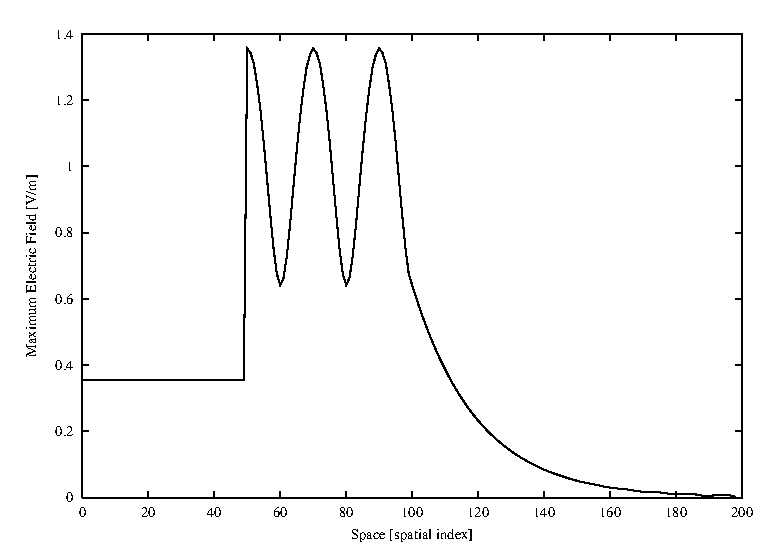
\epsfig{width=4.2in,file=Code/Fdtd-dimensionless/envelope.eps} \\
  (a) \\ \vspace{.2in}
  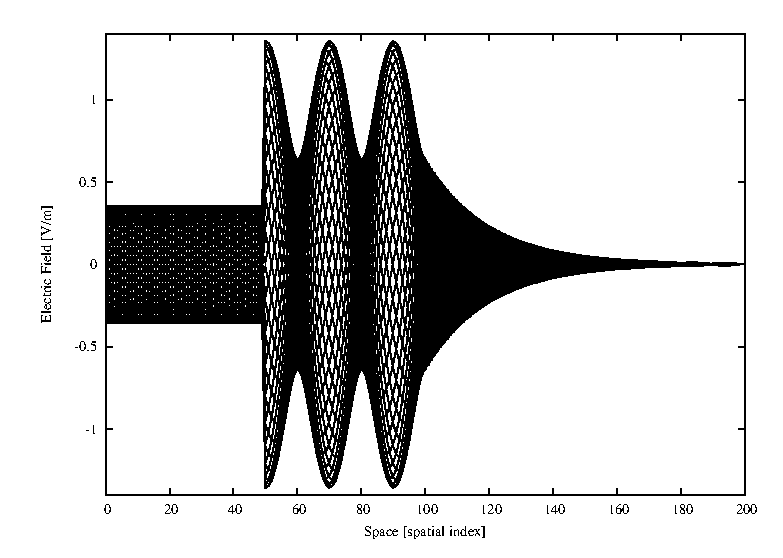
\epsfig{width=4.2in,file=Code/Fdtd-dimensionless/all-snapshots.eps}
  \\ (b) \end{center} \caption{(a) Maximum electric field magnitude
  that exists at each point (obtained by obtaining the maximum value
  in all the snapshots).  The flat line over the first $50$ nodes
  corresponds to the scattered-field region.  The reflected field
  travels without decay and hence produces the flat line.  The
  total-field region between nodes $50$ and $100$ contains a
  standing-wave pattern caused by the interference of the incident and
  scattered fields.  There is exponential decay of the fields beyond
  node $100$ which is where the lossy layer starts.  (b) Superposition
  of $41$ individual snapshots of the field which illustrates the
  envelope of the field.}  \label{fig:decayDemo}
\end{figure}

% Figure generate with using matlab with following commands:
% z=readOneD('sim');
% for i=1:200              
%   zmax(i)=max(abs(z(:,i)));
% end                      
% plot(zmax)
% xlabel('Space [spatial index]')
% ylabel('Maximum of Electric Field Magnitude')

If one were interested in non-zero magnetic conductivity $\sigma_m$,
the loss term which appears in the magnetic-field update equations is
$\sigma_m\Delt/2\mu$.  This term can be handled in exactly the same
way as the term resulting from electric conductivity.  


\section[Transmission Coefficient for a Planar Interface]%
{Example:  Obtaining the Transmission Coefficient for a Planar
Interface \label{sec:specExampleTrans}}

In this last section, we demonstrate how the transmission coefficient
for a planar dielectric boundary can be obtained from the FDTD method.
This serves to highlight many of the points that were considered in
the previous section.  We will compare the results to the exact
solution.  The disparity between the two provides motivation to
determine the dispersion relation in the FDTD (which is covered in
Chap.\ \ref{chap:dispersion}).

The majority of instructional material concerning electromagnetics is
expressed in terms of harmonic, or frequency-domain, signals.  A
temporal dependence of $\exp(j\omega t)$ is understood and therefore
one only has to consider the spatial variation.  In the frequency
domain, the fields and quantities such as the propagation constant and
the characteristic impedance are represented by complex numbers.
These complex numbers give the magnitude and phase of the value and
will be functions of frequency.  In the following discussion a caret
(hat) will be used to indicate a complex quantity and one should keep
in mind that complex numbers are inherently tied to the frequency
domain.  Given the frequency-domain representation of the field at a
point, the temporal signal is recovered by multiplying by
$\exp(j\omega t)$ and taking the real part.  Thus a 1D harmonic field
propagating in the $+x$ direction could be written in any of these
equivalent forms
\begin{equation}
E_z(x,t) = 
  \Re\!\left[\hE_z^+(x,t)\right]
   = 
  \Re\!\left[\hE_z^+(x)e^{j\omega t}\right]
   = 
  \Re\!\left[\hE_0^+e^{-\hgamma x}e^{j\omega t}\right]
   = 
  \Re\!\left[\hE_0^+e^{-(\alpha+j\beta) x}e^{j\omega t}\right],
\end{equation}
where $\Re[]$ indicates the real part.  $\hE_z^+(x)$ is the
frequency-domain representation of the field (i.e., a phasor that is a
function of position), $\hgamma$ is the propagation constant which has
a real part $\alpha$ and an imaginary part $\beta$, and $\hE_0^+$ is a
complex constant that gives the amplitude of the wave (it is
independent of position; the superscript ``$+$'' is merely used to
emphasize that we are discussing a wave propagating in the $+x$
direction).  Note that if more than a single frequency is present,
$\hE_0^+$ does not need to be the same for each frequency.

More generally, $\hE_0^+$ will be a function of frequency (we could
write this expressly as $\hE_0^+(\omega)$ but the caret implicitly
indicates dependence on frequency).  To construct a temporal that
consists of a multiple frequencies, or even a continuous spectrum of
frequencies, one must sum the contributions from each frequency such
as is done with a Fourier integral.

In FDTD simulations the time-domain form of the signal is obtained
directly.  However, one often is interested in the behavior of the
fields as a function of frequency.  As has been discussed in Sec.\
\ref{sec:fftMapping}, one merely has to take the Fourier transform of
a signal to obtain its spectral content.  This transform, by itself,
is typically of little use.  One has to normalize the signal in some
way.  Knowing what came out of a system is rather meaningless unless
one knows what went into the system.  Here we will work through a
couple of simple examples to illustrate how a broad range of spectral
information can be obtained from FDTD simulations.

\subsection[Transmission through Planar Interface]{Transmission through a
Planar Interface (Continuous World) \label{sec:contTrans}}

Consider the planar interface at $x=0$ between two media as depicted
in Fig.\ \ref{fig:planarInterface}.  We restrict consideration to
electric polarization in the $z$ direction and assume the incident
field originates in the first medium.
\begin{figure}
  \begin{center}
    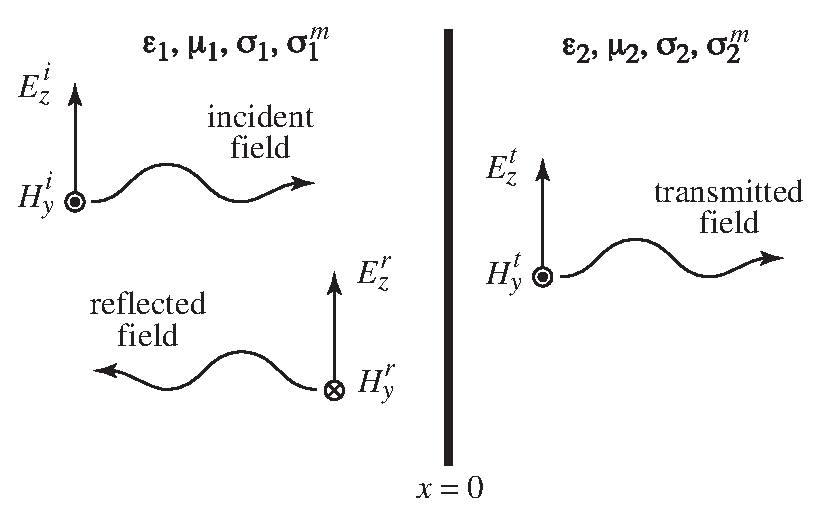
\epsfig{width=3.75in,%
            file=Figures/Fdtd-dimensionless/planar-interface.eps}
  \end{center}
  \caption{Planar interface between two media.  The interface is at
 $x=0$ and a wave is incident on the interface from the left.  When the
 impedances of the two media are not matched, a reflected wave must
 exist in order to satisfy the boundary conditions.}
  \label{fig:planarInterface}
\end{figure}
In the frequency domain, the incident, reflected, and transmitted
fields are given by
\begin{eqnarray}
  \hE_z^i(x) \!&=&\! \hE_{a1}^+ e^{-\hgamma_1 x} 
    \qquad \mbox{\hspace{.92in}incident},\\
  \hE_z^r(x) \!&=&\! \hE_{a1}^- e^{+\hgamma_1 x} =
                   \hG \hE_{a1}^+ e^{+\hgamma_1 x} \qquad \mbox{reflected},\\
  \hE_z^t(x) \!&=&\! \hE_{a2}^+ e^{-\hgamma_2 x} =
                   \hT \hE_{a1}^+ e^{-\hgamma_2 x} \qquad \mbox{transmitted},
\end{eqnarray}
where $\hG$ is the reflection coefficient, $\hT$ is the transmission
coefficient, and $\hgamma_n$ is the propagation constant given by
$j\omega\sqrt{\mu_n(1-j\sigma^m_n/\omega\mu_n)
  \epsilon_n(1-j\sigma_n/\omega\epsilon_n)}$ where the $n$ indicates
the medium and $\sigma^m$ is the magnetic conductivity.  The amplitude
of the incident field $\hE_{a1}^+$ is, in general, complex and a
function of frequency.  By definition $\hG$ and $\hT$ are
\begin{eqnarray}
  \hG &=& \left.\frac{\hE_z^r(x)}{\hE_z^i(x)}\right|_{x=0} =
              \frac{\hE_{a1}^-}{\hE_{a1}^+}, \\
       \hT &=& \left.\frac{\hE_z^t(x)}{\hE_z^i(x)}\right|_{x=0} = 
              \frac{\hE_{a2}^+}{\hE_{a1}^+}.
\end{eqnarray}
The fact that these are defined at $x=0$ is important.

The magnetic field is related to the electric field by
\begin{eqnarray}
  \hH_y^i(x) &=& -\frac{1}{\heta_1}\hE_z^i(x), \\ 
  \hH_y^r(x) &=& \frac{1}{\heta_1}\hE_z^r(x), \\ 
  \hH_y^t(x) &=& -\frac{1}{\heta_2}\hE_z^t(x),
\end{eqnarray}
where the characteristic impedance $\heta_n$ is given by
$\sqrt{\mu_n(1-j\sigma^m_n/\omega\mu_n)/
  \epsilon_n(1-j\sigma_n/\omega\epsilon_n)}$.  Since the magnetic and
electric fields are purely tangential to the planar interface, the sum
of the incident and reflected field at $x=0$ must equal the
transmitted field at the same point.  Matching the boundary condition
on the electric field yields
\begin{equation}
  1 + \hG = \hT,
  \label{eq:matchingFields}
\end{equation}
while matching the boundary conditions on the magnetic field produces
\begin{equation}
 \frac{1}{\heta_1}(1 - \hG) = \frac{1}{\heta_2}\hT.
\end{equation}
Solving these for $\hT$ yields
\begin{equation}
  \hT = \frac{2\heta_2}{\heta_1+\heta_2}.
  \label{eq:transCoefSpectral}
\end{equation}
Using this in \refeq{eq:matchingFields} the reflection coefficient is
found to be
\begin{equation}
  \hG = \frac{\heta_2-\heta_1}{\heta_2+\heta_1}.
  \label{eq:refCoefSpectral}
\end{equation}

\subsection{Measuring the Transmission Coefficient Using FDTD
\label{sec:measureTrans}}

Now consider two FDTD simulations.  The first simulation will be used
to record the incident field.  In this simulation the computational
domain is homogeneous and the material properties correspond to that
of the first medium.  The field is recorded at some observation point
$x_1$.  Since nothing is present to interfere with the incident field,
the recorded field will be simply the incident field at this location,
i.e, $E_z^i(x_1,t)$.  In the second simulation, the second medium is
present.  We record the fields at the same observation point but we
ensure the point was chosen such that it is located in the second
medium (i.e., the interface is to the left of the observation point).
Performing an FDTD simulation in this case yields the transmitted
field $E_z^t(x_1,t)$.  The goal now is to obtain the transmission
coefficient using the temporal recordings of the field obtained from
these two simulations.

{\em Note} that in this section we will not distinguish between the
way in which field propagate in the continuous world and the way in
which they propagate in the FDTD grid.  In
Chap.\ \ref{chap:dispersion} we will discuss in some detail how these
differ.

One cannot use $E_z^t(x_1,t)/E_z^i(x_1,t)$ to obtain the transmission
coefficient.  The transmission coefficient is inherently a
frequency-domain concept and currently we have time-domain signals.
The division of these temporal signals is essentially meaningless
(e.g., the result is undefined when the incident signal is zero).

The incident and transmitted fields must be converted to the frequency
domain using a Fourier transform.  Thus one obtains
\begin{eqnarray}
 \hE_z^i(x_1) &=& {\cal F}\left(E_z^i(x_1,t)\right), \\
 \hE_z^t(x_1) &=&  {\cal F}\left(E_z^t(x_1,t)\right),
\end{eqnarray} 
where ${\cal F}$ indicates the Fourier transform.  The division of
these two functions {\em is} meaningful---at least at all frequencies
where $\hE_z^i(x_1)$ is non-zero.  (At frequencies where
$\hE_z^i(x_1)$ is zero, there is no incident spectral energy and hence
one cannot obtain the transmitted field at those particular
frequencies.  In practice it is relatively easy to introduce energy
into an FDTD grid that spans a broad range of frequencies.)

Since the observation point was not specified to be on the boundary,
the ratio of these field fields is
\begin{equation}
  \frac{\hE_z^t(x_1)}{\hE_z^i(x_1)} =
  \frac{\hE_{a2}^+e^{-\hgamma_2 x_1}}{\hE_{a1}^+e^{-\hgamma_1 x_1}} =
  \frac{\hE_{a2}^+}{\hE_{a1}^+}e^{(\hgamma_1-\hgamma_2) x_1} =
  \hT e^{(\hgamma_1-\hgamma_2) x_1}.
\end{equation}
Solving this for $\hT$ yields
\begin{equation}
  \hT(\omega) = e^{(\hgamma_2-\hgamma_1) x_1}
  \frac{\hE_z^t(x_1)}{\hE_z^i(x_1)}.
  \label{eq:transCoefShifted}
\end{equation}

To demonstrate how the transmission coefficient can be
reconstructed from FDTD simulations, let us consider an example where
the first medium is free space and the second one has a relative
permittivity $\epsilon_r$ of $9$.  In this case
$\hgamma_1=j\omega\sqrt{\mu_0\epsilon_0}=j\beta_0$ and
$\hgamma_2=j\omega\sqrt{\mu_0 9\epsilon_0}=j3\beta_0$.
Therefore \refeq{eq:transCoefShifted} becomes
\begin{equation}
  \hT(\omega) = e^{j(3\beta_0-\beta_0) x_1}
  \frac{\hE_z^t(x_1)}{\hE_z^i(x_1)}
  = e^{j2\beta_0 x_1}
  \frac{\hE_z^t(x_1)}{\hE_z^i(x_1)}.
\end{equation}
The terms in the exponent can be written
\begin{equation}
  2\beta_0 x_1 = 2\frac{2\pi}{\lambda}x_1 = 
  \frac{4\pi}{\ppw\Delx}N_1\Delx =
  \frac{4\pi}{\ppw}N_1
  \label{eq:transExponent}
\end{equation}
where $N_1$ is the number of spatial steps between the interface and
the observation point at $x_1$ and, as was discussed in Chap.\
\ref{chap:dimensionless}, $\ppw$ is the number of spatial steps per a
free-space wavelength of $\lambda$.

The continuous-world transmission coefficient can be calculated quite
easily from \refeq{eq:transCoefSpectral} and this provides a reference
solution.  Ideally the FDTD simulation would yield this same value for
all frequencies.  For this particular example the characteristic
impedance of the first medium is $\heta_1=\eta_0$ while for the second
medium it is $\heta_2=\eta_0/3$.  Thus the transmission coefficient
is
\begin{equation}
  \hT_{\mbox{\scriptsize exact}} = \frac{2\eta_0/3}{\eta_0+\eta_0/3} = 1/2.
  \label{eq:transExact}
\end{equation}
Note that this is a real number and independent of frequency (so the
tilde on $T$ is somewhat misleading).

For the FDTD simulations, let us record the field 80 spatial steps
away from the interface, i.e., $N_1=80$, and run the simulation for
8192 time steps, i.e., $N_T=8192$.  The simulation is run at the
Courant limit $S_c=1$.  The source is a Ricker wavelet discretized so
that the peak spectral content exists at 50 points per wavelength
($N_P=50$).  From Sec.\
\ref{sec:fftMapping}, recall the relationship between the points per
wavelength $\ppw$ and frequency index $N_{\mathrm{freq}}$ which is
repeated below:
\begin{equation}
  N_{\mathrm{freq}} = \frac{N_T}{\ppw} S_c.
\end{equation}
With a Courant number of unity and 8192 time steps, the points per
wavelength for any given frequency (or spectral index) is given by
\begin{equation}
  \ppw = \frac{8192}{N_{\mathrm{freq}}}.
\end{equation}
Combining this with \refeq{eq:transCoefShifted} and
\refeq{eq:transExponent} yields
\begin{equation}
  \hT_{\mbox{\scriptsize FDTD}}
  = e^{j\left(\frac{4\pi N_1N_{\mathrm{freq}}}{8192}\right)}
  \frac{\hE_z^t(x_1)}{\hE_z^i(x_1)}.
  \label{eq:transFDTD}
\end{equation}

Ideally \refeq{eq:transExact} and \refeq{eq:transFDTD} will agree at
all frequencies.  To see if that is the case, Fig.\
\ref{fig:incTransFields} shows three plots related to the incident and
transmitted fields.  Figure \ref{fig:incTransFields}(a) shows the
first 500 time steps of the temporal signals recorded at the
observation point both with and without the interface present
(i.e., the transmitted and incident fields, respectively).  Figure
\ref{fig:incTransFields}(b) shows the magnitude of the Fourier
transforms of the incident and transmitted fields for the first 500
frequencies.  Since a Ricker wavelet was used, the spectra are
essentially in accordance with the discussion of Sec.\
\ref{sec:ricker}.  There is no spectral energy at dc and the spectral
content exponentially approaches zero at high frequencies.

\begin{figure}
  \begin{center}
   \epsfig{width=5.4in,file=Code/Fdtd-spectral/fields.eps}
  \end{center}

  \caption{(a) Time-domain fields at the observation point both with
   and the without the interface present.  The field without the
   interface is the incident field and the one with the interface is
   the transmitted field.  (b) Magnitude of the Fourier transforms of
   the incident and transmitted fields.  The transforms are plotted
   versus the frequency index $N_{\mathrm{freq}}$.  It can be seen that
   the fields do not have much spectral content near dc nor at high
   frequencies.  (c) Magnitude of the transmitted field normalized by
   the incident field versus the frequency index.  Ideally this would
   be $1/2$ for all frequencies.  Errors are clearly evident when the
   spectral content of the incident field is small.}
   \label{fig:incTransFields}
\end{figure}

Figure \ref{fig:incTransFields}(c) plots the magnitude of the ratio of
the transmitted and incident field as a function of frequency.
Ideally this would be $1/2$ for all frequencies.  Note the rather
small vertical scale of the plot.  Near dc the normalized transmitted
field differs rather significantly from the ideal value, but this is
in a region where the results should not be trusted because there is
not enough incident energy at these frequencies.  At the higher
frequencies some oscillations are present.  The normalized field
generally remains within two percent of the ideal value over this
range of frequencies.

Figure \ref{fig:transCoefVsFreq}(a) provides the same information as
Fig.\ \ref{fig:incTransFields}(c) except now the result is plotted
versus the discretization $\ppw$.  In this figure dc is off the scale
to the right (since in theory dc has an infinite number of points per
wavelength).  As the frequency goes up, the wavelength gets shorter
and hence the number of points per wavelength decreases.  Thus high
frequencies are to the left and low frequencies are to the right.  The
highest frequency in this plot corresponds to an $N_{\mathrm{freq}}$
of $500$.  In terms of the discretization, this is
$N_\lambda=N_T/N_{\mathrm{freq}}=16.384$.  This may not seem like a
particularly coarse discretization, but one needs to keep in mind that
this is the discretization in frees pace.  Within the dielectric, which
here has $\epsilon_r=9$, the wavelength is three times smaller and
hence within the dielectric the fields are only discretized at
approximately five points per wavelength (which is considered a very
coarse discretization).  From this figure it is clear that the FDTD
simulations provide results which are close to the ideal over a fairly
broad range of frequencies.

\begin{figure}
  \begin{center}
   \epsfig{width=5.4in,file=Code/Fdtd-spectral/trans-coef.eps}
  \end{center}
  \caption{(a) The magnitude of the normalized transmitted field as a
    function of the (free space) discretization $N_\lambda$.  Ideally
    this would be $1/2$ for all discretizations. (b) Real and
    imaginary part of the transmission coefficient transformed back to
    the interface $x=0$ versus discretization.  Ideally the real part
    would be $1/2$ and the imaginary part would be zero for all
    discretization.  For these plots the observation point was $80$
    cells from the interface ($N_1 = 80$).
   \label{fig:transCoefVsFreq}}
\end{figure}

Figure \ref{fig:transCoefVsFreq}(b) shows the real and imaginary part of
the reflection coefficient, i.e., $\hT_{\mbox{\scriptsize FDTD}}$
defined in \refeq{eq:transFDTD}, as a function of the discretization.
Ideally the imaginary part would be zero and the real part would be
$1/2$.  As can be seen, although the magnitude of the transmission
coefficient is nearly $1/2$ over the entire spectrum, the phase differs
rather significantly as the discretization decreases (i.e., the
frequency increases).  

The Matlab code used to generate Fig.\ \ref{fig:incTransFields} is
shown in Program \ref{pro:transformFields} while the code which
generated Fig.\ \ref{fig:transCoefVsFreq} is given in Program
\ref{pro:transCoefficient}.  It is assumed the incident field from the
FDTD simulation is recorded to a file named {\tt inc-8192} while the
transmitted field, i.e., the field when the dielectric is present, is
recorded in {\tt die-8192}.  The code in Program
\ref{pro:transformFields} has to be run prior to that of 
\ref{pro:transCoefficient} in order to load and initialize the data.

Let us now consider the same scenario but let the observation point be
four steps away from the boundary instead of $80$, i.e., $N_1=4$.
Following the previous steps, the incident and transmitted fields are
recorded, their transforms are taken, then divided, and finally the
phase is adjusted to obtain the transmission coefficient.  The result
for this observation point is shown in Fig.\
\ref{fig:transCoefVsFreqX4}.  The real and imaginary parts stay closer
to the ideal values over a larger range of frequencies than when the
observation point was $80$ cells from the boundary.  The fact that the
quality of the results are frequency sensitive as well as sensitive to
the observation point is a consequence of numeric dispersion in the
FDTD grid, i.e., different frequencies propagate at different speeds.
(This is the subject of Chap.\ \ref{chap:dispersion}.)
\begin{figure}
  \begin{center}
   \epsfig{width=5.4in,file=Code/Fdtd-spectral/trans-coef-x4.eps}
  \end{center}

  \caption{Real and imaginary part of the transmission coefficient
    transformed back to the interface $x=0$ versus discretization.
    Ideally the real part would be $1/2$ and the imaginary part would
    be zero for all discretization.  The observation point was four
    cells from the interface ($N_1 = 4$).}
   \label{fig:transCoefVsFreqX4}
\end{figure}

\begin{program}
Matlab session used to generate Fig.\ \ref{fig:incTransFields}.
 \label{pro:transformFields}
\codemiddle
\begin{lstlisting}[language=Matlab]
incTime = dlmread('inc-8192'); % incident field file
dieTime = dlmread('die-8192'); % transmitted field file

inc = fft(incTime);  % take Fourier transforms
die = fft(dieTime);

nSteps = length(incTime);  % number of time steps
freqMin = 1;    % minimun frequency index of interest
freqMax = 500;  % maximum frequency of interest
freqIndex = freqMin:freqMax; % range of frequencies of interest
% correct for offset of 1 in matlab's indexing
freqSlice = freqIndex + 1;
courantNumber = 1;
% points per wavelength for freqencies of interest
nLambda = nSteps ./ freqIndex * courantNumber;
clf
subplot(3, 1, 1)
hold on
plot(incTime(freqSlice), '-.');
plot(dieTime(freqSlice));
legend('Incident field', 'Transmitted field');
xlabel('Temporal Index');
ylabel('{\it E_z}[{\it x}_1,{\it t}] V/m');
title('(a) Temporal Fields');

subplot(3,1,2)
hold on
plot(freqIndex, abs(inc(freqSlice)), '-.');
plot(freqIndex, abs(die(freqSlice)));
legend('Incident field', 'Transmitted field');
xlabel('Frequency Index');
ylabel('|{\it E_z}[{\it x}_1,\omega]|');
title('(b) Transform vs. Frequency Index');
hold off

subplot(3, 1, 3)
hold on
plot(freqIndex, abs(die(freqSlice) ./ inc(freqSlice)));
xlabel('Frequency Index');
ylabel('|{\it E^t_z}[{\it x}_1,\omega]/...
                          {\it E^i_z}[{\it x}_1,\omega]|');
title('(c) Normalized Transmitted Field vs. Frequency Index');
hold off
\end{lstlisting}
\end{program}

\begin{program}
Matlab session used to generate Fig.\
\ref{fig:transCoefVsFreq}.  The commands shown in Program
\ref{pro:transformFields} would have to be run prior to these
commands in order to read the data, generate the Fourier transforms, etc.
 \label{pro:transCoefficient}
\codemiddle
\begin{lstlisting}[language=Matlab]
clf

subplot(2, 1, 1)
hold on
plot(nLambda, abs(die(freqSlice) ./ inc(freqSlice)));
xlabel('Points per Wavelength');
ylabel('|{\it E^t_z}[{\it x}_1,\omega]/...
                          {\it E^i_z}[{\it x}_1,\omega]|');
title('(a) Normalized Transmitted Field vs. Discretization');
axis([0 300 0 1])
hold off

% Array obtained from exp() must be transposed to make arrays
% conformal.  Simply using ' (a prime) for trasposition will yield
% the conjugate transpose.  Instead, use .' (dot-prime) to get
% transposition without conjugation.
subplot(2, 1, 2)
hold on
plot(nLambda, real(exp(j*pi*freqIndex/25.6).' .* ...
                   die(freqSlice) ./ inc(freqSlice)));
plot(nLambda, imag(exp(j*pi*freqIndex/25.6).' .* ...
                   die(freqSlice) ./ inc(freqSlice)), '-.');
xlabel('Points per Wavelength');
ylabel('Transmission Coefficient, {\it T}(\omega)');
title('(b) Real and Imaginary Part of Transmission Coefficient');
legend('Real part', 'Imaginary part');
axis([0 300 -1 1])
grid on
hold off
\end{lstlisting}
\end{program}

Although we have only considered the transmission coefficient in this
example, the reflection coefficient could be obtained in a similar
fashion.  We have intentionally considered a very simple problem in
order to be able to compare easily the FDTD solution to the exact
solution.  However one should keep in mind that the FDTD method could
be used to analyze the reflection or transmission coefficient for a
much more complicated scenario, e.g., one in which the material
properties varied continuously, and perhaps quite erratically (with
some discontinuities present), over the transition from one half-space
to the next.  Provided a sufficiently small spatial step-size was
used, the FDTD method can solve this problem with essentially no more
effort than was used to model the abrupt interface.  However, to
obtain the exact solution, one may have to work much harder.
